
\chapter{RSA Signatures}
\label{chap:rsa}

In this chapter, we will discuss the RSA digital-signature scheme.
The RSA paper\autocite{RSA} was tremendously influential because it gave
the first constructions of digital signatures and public-key encryption.
(We will talk about public-key encryption in detail later on.)

The RSA cryptosystem is going out of style for a few reasons: 
generating RSA keys is relatively expensive and the keys are relatively large
(4096 bits for RSA versus 256 bits for more modern elliptic-curve-based cryptosystems).
In addition, a large-scale quantum computer could---in theory, at least---break
RSA-style cryptosystems.

The RSA cryptosystem is worth studying for a few reasons:
\begin{itemize}
  \item RSA's security is related to the problem of factoring large integers,
        which is (arguably) the most natural ``hard'' computational problem
        out there.
       
  \item RSA gives the only known instantiation of a \emph{trapdoor one-way permutation},
        which we will define shortly.

  \item RSA has a number of esoteric properties that are useful for advanced
        cryptographic constructions. For example, it gives a ``group of unknown order.''
        See
    \href{https://toc.cryptobook.us/book.pdf#page=436}{Boneh-Shoup, Chapter 10.9} for details.

  \item RSA signatures are used on the vast majority of public-key certificates today.\footnote{As
    of today, around 94\% of certificates in the Certificate Transparency logs use RSA signatures:
\url{https://ct.cloudflare.com/}.}

The most commonly used type of RSA signatures (``PKCS \#1 v1.5'') is
more complicated---and no more secure---than the
construction we describe here, but that
construction is still used for historical reasons.

\end{itemize}

\section{Trapdoor one-way permutations}

\begin{figure}
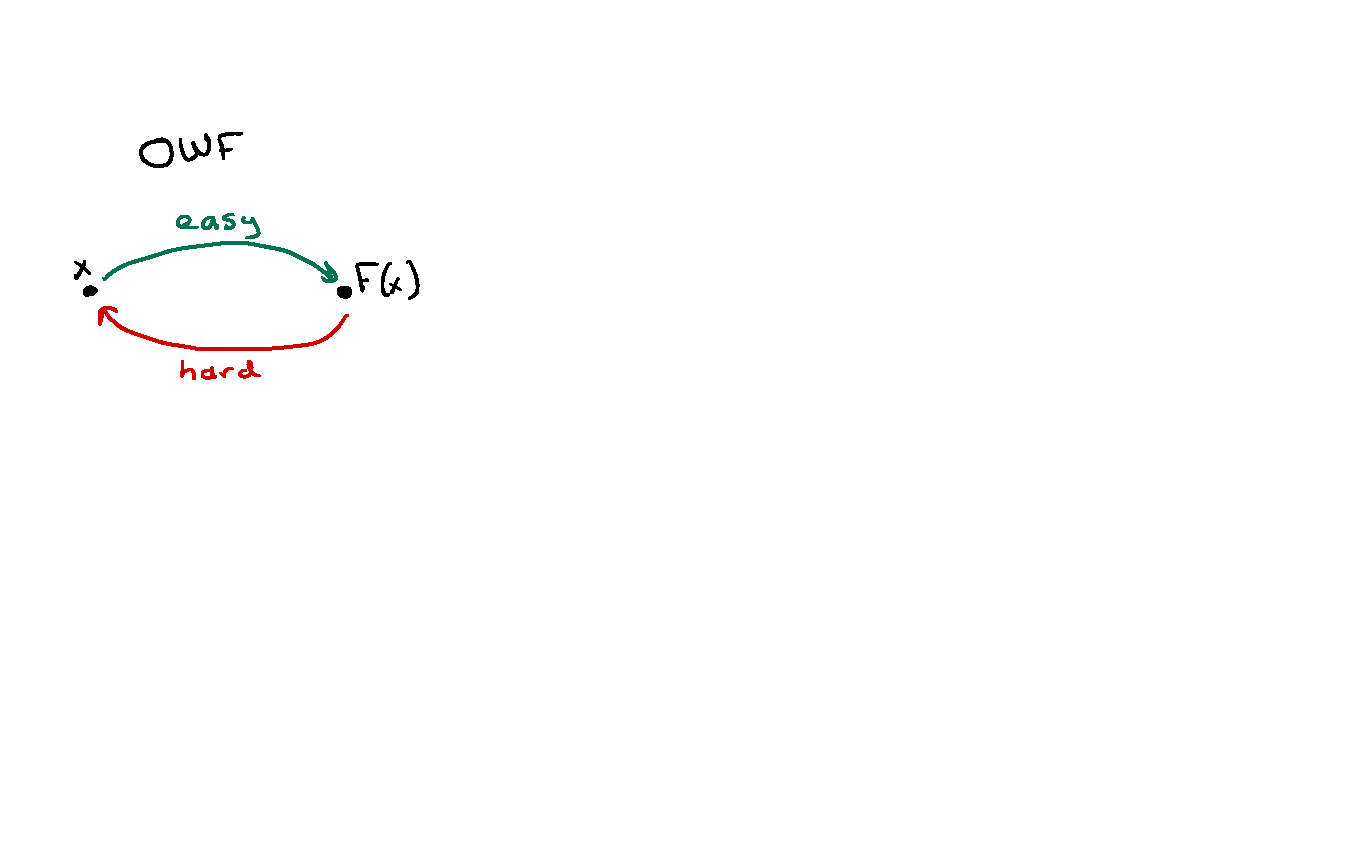
\includegraphics[width=0.45\textwidth]{figs/rsa-owf.pdf}
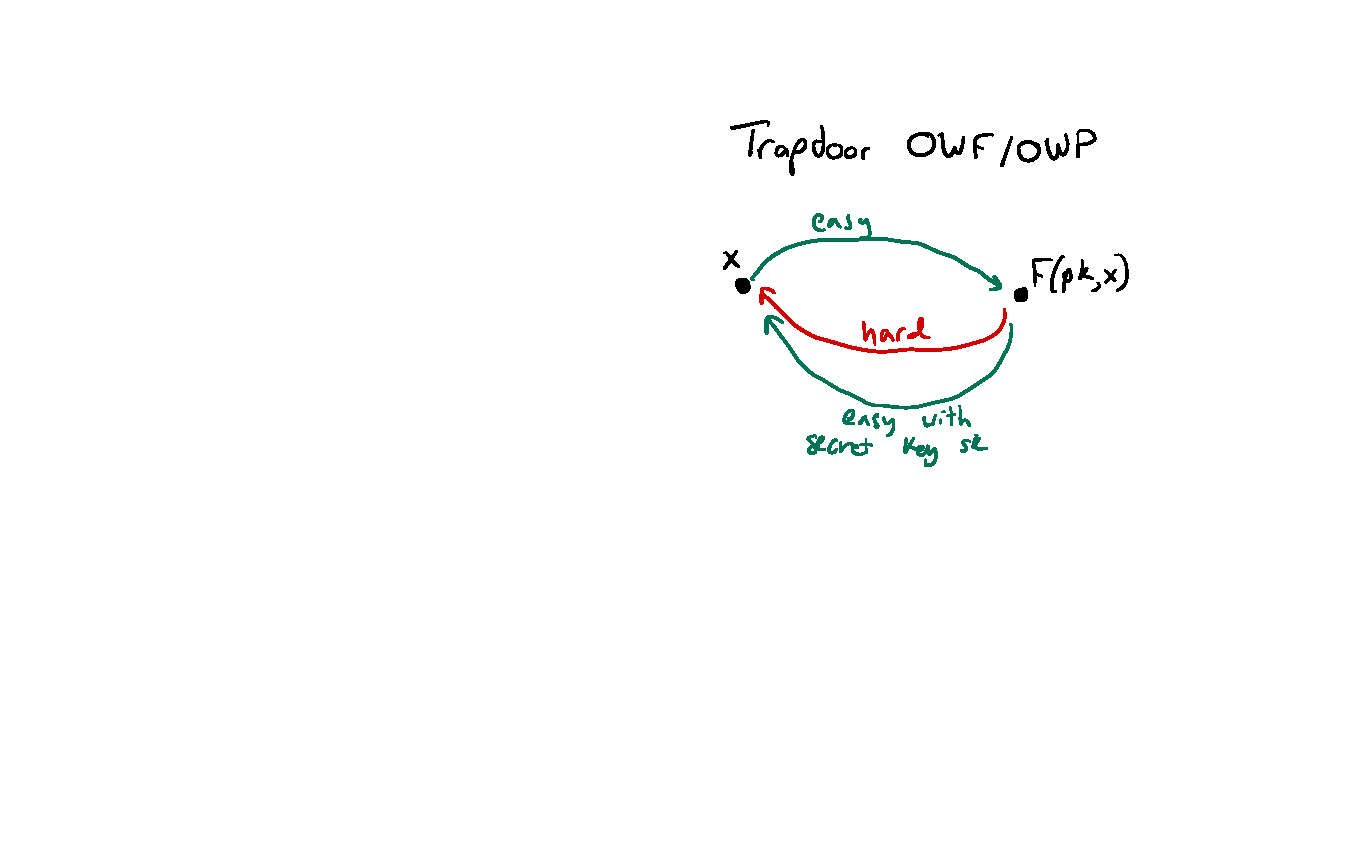
\includegraphics[width=0.55\textwidth]{figs/rsa-trapdoor.pdf}
\caption{A one-way function (at left) is hard to invert on random inputs.
A trapdoor one-way function/permutation (at right) is a function keyed
by a public key. The function is easy to invert given the secret key 
and is hard to invert otherwise.
}
\end{figure}

RSA implements a \emph{trapdoor one-way function}.
Informally, a trapdoor one-way function is a function that is
easy to compute in the forward direction but that is hard to 
invert \emph{except} to someone knowing a secret key.
So it is like a one-way function with a ``trapdoor'' that allows
efficient inversion.

RSA actually implements a trapdoor one-way \emph{permutation}---that is,
it maps an input space onto itself with no collisions.

\subsection{Definition}

Formally, a trapdoor one-way permutation over input space $\calX$ is a triple of
efficient algorithms:\marginnote{If we wanted to be completely formal, the
input space would be parameterized by the security parameter $\lambda$.
So we would have a family of input spaces $\{\calX_\lambda\}_{\lambda \in \N}$---%
one for each choice of $\lambda$. This way the input space can grow with~$\lambda$.}

\begin{itemize}
  \item $\Gen(1^\lambda) \to (\sk, \pk)$.
        The key-generation algorithm takes as input the security parameter $\lambda \in \N$,
        expressed as a unary string, and outputs a secret key and a public key.
  \item $F(\pk, x) \to y$.\marginnote{In the RSA construction, the input space $\calX$
depends on the public key, but we elide that technical detail here.}
        The evaluation algorithm $F$ takes as input the
        public key $\pk$ and an input $x \in \calX$, and outputs 
        a value $y \in \calX$.
  \item $I(\sk, y) \to x'$.
        The inversion algorithm $I$ takes as input the secret key $\sk$
        and a point $y \in \calX$, and outputs its inverse $x \in \calX$.
\end{itemize}

\paragraph{Correctness.}
Informally, we want that for keypairs $(\sk, \pk)$ output by $\Gen$,
we have that $F(\pk, \cdot)$ and $I(\sk, \cdot)$ are inverses of each other.
More formally, for all $\lambda \in \N$, $(\sk, \pk) \gets \Gen(1^\lambda)$, and $x \in \calX$,
we require:
\[ I(\sk, F(\pk, x))= x.\]

\paragraph{Security.}
Security requires that $F(\pk, \cdot)$ is hard to invert (in the sense of a one-way function)
on a randomly sampled input in the input space $\calX$, even when the adversary 
is given the public key $\pk$.
That is, for all efficient adversaries $\calA$, there exists a negligible function $\negl(\cdot)$
such that 
\[ \Pr\left[ 
\calA(\pk, F(\pk, x)) = x
\colon \begin{aligned}
  (\sk, \pk) &\gets \Gen(1^\lambda)\\
  x &\getsr \calX
\end{aligned}\right] \leq \negl(\lambda).\]

When we use the RSA cryptosystem, we make the assumption 
that the RSA function is hard to invert given only the public key:
\begin{defn}[RSA Assumption]
The RSA function $(\Gen, F, I)$ is a trapdoor one-way permutation.
\end{defn}

\paragraph{\textbf{IMPORTANT}:}
Just as a one-way function is only hard to invert on a \emph{randomly sampled input},
a trapdoor one-way function is only hard to invert on a randomly sampled input.
Many of the cryptographic failures of RSA come from assuming that the RSA
one-way function is hard to invert on non-random inputs.


\subsection{Digital signatures from trapdoor one-way permutations}

This construction is called ``full-domain hash.''\autocite{BR93}
The construction makes use of a hash function $H$ and resulting
signature scheme is secure, provided that we model the hash function~$H$
as a ``random oracle.''

In other words, to argue security, it is not sufficient to show that
$H$ is, for example, collision resistant.
Instead, we can only prove security provided that we pretend that $H$
is a truly random function---i.e., in the random-oracle model.
When we instantiate the hash function $H$ with some concrete cryptographic
hash function, such as SHA256, we hope that the resulting signature
scheme is still secure.
In practice, this approach works quite well.

One way to think about it is that if a signature scheme is secure
in the random-oracle model, then the concrete signature scheme
is in some sense secure against attacks that do not exploit the peculiarities
of the hash function.

\medskip 

In the construction, we use:
\begin{itemize}
  \item a trapdoor one-way permutation $(\Gen, F, I)$, and
  \item a hash function $H \colon \zo^* \to \calX$,
        which we model as a random oracle in the
        security analysis.
\end{itemize}

\paragraph{Construction.}
We construct a digital-signature scheme $(\Gen, \Sign, \Ver)$ as follows:
\begin{itemize}
  \item $\Gen$ -- Just run the key-generation algorithm for the
        trapdoor one-way permutation.
  \item $\Sign(\sk, m) \to \sigma$.
        Hash the message down to an element $h$ of the input space $\calX$
        of the trapdoor one-way permutation using the hash function $H$. Then invert
        the trapdoor one-way permutation at that point:
        \begin{itemize}
          \item Compute $h \gets H(m)$.
          \item Output $\sigma \gets I(\sk, h)$.
        \end{itemize}
      \item $\Ver(\pk, m, \sigma) \to \zo.$ 
        \begin{itemize}
          \item Compute $h' \gets H(m)$.
          \item Accept if $F(\pk, \sigma) = h'$.
        \end{itemize}
\end{itemize}

Notice that the use of a hash function here is \textbf{critical} to
security, since (in the random oracle) it means that forging a signature
is as hard as inverting $F$ on a random point in its co-domain.
Without the hash function, forging a signature is only as hard as 
inverting $F$ on an attacker-chosen point in its co-domain, which 
could be easy.

\paragraph{Correctness.}
For all $\lambda \in \N$, $(\sk, \pk) \gets \Gen(1^\lambda)$, and $m \in \zo^*$,
we have:
\begin{align*}
\Ver(\pk, m, \Sign(\sk, m)) &= 1\{ F(\pk, I(\sk, H(m))) = H(m) \}\\
&= 1\{ I(\sk, F(\pk, I(\sk, H(m)))) = I(\sk, H(m)) \}
\intertext{and by correctness of the trapdoor one-way permutation:}
&= 1\{ I(\sk, H(m)) = I(\sk, H(m)) \} = 1.
\end{align*}

\paragraph{Security.}
The intuition here is that if the adversary cannot invert $F$,
it cannot find the preimage of $H(m)$ under $F$ for any message
on which it has not seen a signature.
See \href{https://toc.cryptobook.us/book.pdf#page=550}{Boneh-Shoup Chapter 13.3}
for the full security analysis.

\section{The RSA construction: Forward direction}

The algorithms for 
key-generation and 
for evaluating the RSA permutation
in the forward direction are not too complicated.

In what follows, we present RSA with 
public exponent $e=5$.
The same construction works with many other choices of $e$,
just by replacing all of the ``5''s below with some other
small prime: 3, 7, 13, etc.
A popular choice of the public exponent $e$ in practice is $e=2^{16}+1$.
The complexity of computing the RSA function in the forward
direction scales with the size of $e$, so we prefer small
choices of $e$.

\begin{itemize}
  \item $\Gen(1^\lambda) \to (\sk, \pk)$.\marginnote{In practice,
    we usually take the bitlength of primes to be $\lambda=1024$
    or $\lambda = 2048$.}
  \begin{itemize}
    \item Sample two random $\lambda$-bit primes $p$ and $q$
      such that $p \equiv q \equiv 4 \pmod 5$.\marginnote{%
        Standard RSA implementations require
        the weaker condition that the public exponent $e$
        shares no prime factors with $p-1$ and $q-1$.
        Using the stronger condition here simplifies 
        the inversion algorithm.}
    \item Set $N \gets p \cdot q$.
    \item Output $\sk \gets (p, q)$, and $\pk = N$.
  \end{itemize}
  \item $F(\pk = N, x) \to y$.
\begin{itemize}
  \item The input space for the RSA function is \\
    $\calX = \Z^*_N$---the set of elements in $\{0, 1, 2, \dots, N-1\}$
    relatively prime to $N$.
    \item Output $y \gets x^5 \bmod N$.
\end{itemize}
\end{itemize}

\begin{remark}
The key-generation algorithm relies on us being able
to sample large random primes.
One perhaps surprising fact is that there are many many 
large primes.
In particular, if you pick a random $\lambda$-bit number,
the probability that it is prime is roughly $1/\lambda$.\marginnote{For more 
on this, look up the Prime Number Theorem.}

We can sample a random $\lambda$-bit prime by just
picking random integers in the range $[2^\lambda, 2^{\lambda + 1})$
until we find a prime.
We can test for primality in $\approx \lambda^4$ time using
the Miller-Rabin primality test.
We also need that there are infinitely many primes congruent to
$4 \bmod 5$, but fortunately there are.
Generating RSA keys is expensive---it can take
a few seconds even on a modern machine.
\end{remark}

Notice that computing the RSA function in the forward direction is
relatively fast: it just requires three multiplications 
modulo a 2048-bit number $N$. That is, to compute $x^5 \bmod N$, we compute:
\[ (x^2)^2 \cdot x = x^5\mod N.\]


\medskip

Before describing the RSA inversion algorithm, we discuss 
why the RSA trapdoor one-way permutation should be hard
to invert without the secret key.

\subsection{Why should the RSA function be hard to invert?}
To invert the RSA function, the attacker's is effectively given
a value $y \getsr \Z_N$ and must find a value $x$ such that $x^5 = y \bmod N$.
Or, put another way, the attacker's task is essentially the following:
\begin{itemize}
  \item \textbf{Given:} A polynomial $p(X) \deq X^5 - y \in \Z_N[X]$,
                        for $y \getsr \Z_N$.
  \item \textbf{Find:}  A value $x \in \Z_N$ such that $p(x) = 0 \in \Z_N$.
\end{itemize}

So the attacker must find the root of a polynomial modulo a composite integer~$N$.

The premise of RSA-style cryptosystems is that we only
know of essentially two ways to find roots of polynomials modulo $N$:
\begin{itemize}
\item \textbf{Factor $N$ into primes} and find a root modulo each of the primes.
      (We will say more on this in a moment.)
      Since the best algorithms for factoring run in time roughly $2^{\sqrt[3]{\log N}} = 2^{\sqrt[3]{\lambda}}$,
      this approach is infeasible at present without knowing the factorization of $N$.

\item \textbf{Find a root over the integers} and reduce it modulo $N$.\marginnote{Actually,
      it suffices to find a root over the rational numbers, but the distinction isn't important here.}
      For example, it is easy to find a root of polynomials such as:\\
\begin{align*}
  X + 4 &= 3 &&\mod N,&\\
  X + 2Y &= 5 &&\mod N,&\\
  X^2 &= 9 &&\mod N\text{, and}&\\
  X^2-3x+2 &= (X-2)(X-1) = 3 &&\mod N.
\end{align*}\marginnote{There are many clever attacks 
for solving polynomial equations modulo composites
that work in certain special cases, but for most purposes
these are the two known attacks.}
When $y \getsr \Z_N$, the probability that $y$ is a perfect
5-th power, and thus that there is an integral root to $X^5 - y$,
is $\sqrt[5]{N}/N \approx 2^{-4\lambda/5}$, which is negligible
in the security parameter~$\lambda$.
So solving this equation over the integers is a dead end.

\paragraph{Is inverting the RSA function as hard as factoring the modulus?}
No one knows---the question has been open since the invention of RSA.
We do know that finding roots of certain polynomial equations, such as
$p(X) \deq X^2 - y \bmod N$ for random $y \getsr \Z_N$ \emph{is} as 
hard as factoring the modulus $N$.
But for RSA-type polynomials, the answer is unclear.

\end{itemize}

\section{The RSA construction: Inverse direction}

To understand how the inversion algorithm works, we will need some
number-theoretic tools.


\subsection{Tools from number theory}
For a natural number $N$, let $\phi(N)$ denote the number of integers
in $\Z_N = \{1, 2, 3, \dots, N\}$ that are relatively prime to $N$.\marginnote{Two
natural numbers are \emph{relatively prime} if they share no prime factors.}
When $p$ is prime $\phi(p) = p-1$.
The function $\phi(\cdot)$ is called \emph{Euler's totient function}.

When $N=pq$ is the product of two distinct primes, $\phi(N) = (p-1)(q-1)$.
That is so because all numbers in $\Z_N$ are relatively prime to $N$ except
$N$ and the multiples of $p$ and $q$:
\[ p, 2p, 3p, \dots, (q-1)p,\ \ \ q, 2q, 3q, \dots, (p-1)q.\]
So there are $N - (q-1) - (p-1) - 1 = (p-1)(q-1)$ numbers
in $\Z_N$ relatively prime to $N$.

\begin{theorem}[Euler's Theorem]\label{thm:euler}
Let $N$ be a natural number. Then for all $a \in \Z^*_N$,
\[ a^{\phi(N)} = 1 \mod N.\]
\end{theorem}
\begin{proof}
Consider the sets $\Z^*_N$ and $\{ax \bmod N \mid x \in \Z^*_N\}$.
These sets are equal, so the product of the elements in the two
sets is equal.
Let $X \gets \prod_{x \in \Z^*_N} x \bmod N$.
Then 
\[ X = a^{\phi(N)}X \bmod N \quad \Rightarrow\quad 1 = a^{\phi(N)} \bmod N.\]
\end{proof}



\begin{lemma}\label{lemma:inv}
Let $p$ and $q$ be distinct primes congruent to $4$ modulo $5$.
Define the integer $d = \frac{\phi(N) - 4}{5} + 1$.
Then $5d \equiv 1 \bmod \phi(N)$.
\end{lemma}

\begin{proof}
Observe that
\[ p \equiv 4 \bmod 5 \quad \Rightarrow \quad \phi(N) - 4 \equiv 0 \bmod 5,\]
so $\frac{\phi(N) - 4}{5}$ is an integer and thus $d$ is well defined.
Then $5 d = \phi(N) - 4 + 5 = 1 \bmod \phi(N)$.
\end{proof}


\subsection{Inverting the RSA function}

With the number theory out of the way, we can now describe how
to invert the RSA function.
All we have to do is to show how to compute a fifth root of $y \bmod N$.

\begin{itemize}
  \item $I(\sk, y) \to x$.
\begin{itemize}
  \item The secret key $\sk$ consists of the prime factors $p,q$ of $N$.
        Recall that $\phi(N) = (p-1)(q-1)$.
  \item Compute the integer $d \gets \frac{\phi(N) - 4}{5} + 1$, as in
    \cref{lemma:inv}.\marginnote{%
    We sometimes call $d$ the \emph{private exponent} in RSA.}

  \item Return $y^d \bmod N$.
\end{itemize}
\end{itemize}

It is not obvious why the inversion algorithm is correct.
Say that $y = x^5 \bmod N$.
Then:
\begin{align*}
  y^d &= (x^5)^d &&\bmod N\\
      &= x^{5d} &&\bmod N\\
&= x^{k \cdot \phi(N) + 1} &&\bmod N, \qquad \text{for some $k \in \Z$, by \cref{lemma:inv}}\\
        &= x \cdot (x^{\phi(N)})^k &&\bmod N\\
&= x &&\bmod N, \qquad\text{by \cref{thm:euler}}.\\
\end{align*}
We could write $5d = k \phi(N) + 1$ because from \cref{lemma:inv},
we know that $5d \equiv 1 \bmod \phi(N)$.

\paragraph{Using other public exponents.}
For our RSA-inversion algorithm to work, we need only to
compute the multiplicative inverse $e$ modulo $\phi(N)$.
That is, we need to compute an integers $d$ such that
$ed \equiv 1 \bmod \phi(N)$.
Such an inverse always exists when $e$ and $\phi(N)=(p-1)(q-1)$ are
relatively prime.
RSA implementations typically use the extended Euclidean
algorithm to compute the multiplicative inverse of $e$ modulo $\phi(N)$.
That algorithm is more general, but the one we used in \cref{lemma:inv}
is simpler and is self-contained.

\paragraph{Inverting RSA is easy on a negligible fraction of points.}
Recall the RSA is 
If the preimage under the RSA function of a point $y$ is very very small,
then 
If $x < N^{1/5}$, then computing $x$ given $y = x^5 \bmod N$ is \emph{easy}.


\paragraph{Is inverting RSA as hard as factoring the modulus $N$?}
The inversion algorithm we showed here requires knowing the prime factors
of the modulus $N$.
Inverting RSA is thus \emph{no harder than} factoring $N$.

Is inverting RSA \emph{as hard as} factoring $N$?
In particular, if we have an efficient algorithm $\calA$ that inverts
RSA, can we use $\calA$ to factor the modulus $N$?
No one knows!

Most cryptographers, I would guess, believe that inverting the RSA function
is as hard as factoring.
But for all we know, it could be that computing fifth roots modulo $N$ is \emph{easier}
than factoring the modulus.


